\documentclass{emulateapj}
\documentclass[12pt,preprint]{aastex}

\usepackage{graphicx}
\usepackage{float}
\usepackage{amsmath}
\usepackage{epsfig,floatflt}
\usepackage{fourier}
\usepackage{listings}
\newcommand{\R}{\mathbb{R}}
\usepackage{subfig}

\lstset{language=python,
    showspaces=false,
    extendedchars=true,
    breaklines=true,
    tabsize=2,
    basicstyle=\small\ttfamily,
    frame=single,
    columns=flexible,
    keepspaces=true,
    }


\DeclareMathAlphabet{\mathcal}{OMS}{cmsy}{m}{n}
\SetMathAlphabet{\mathcal}{bold}{OMS}{cmsy}{b}{n}


\begin{document}

\title{FYS3150 Computational Physics, project 1}

\author{Stig-Nicolai Foyn, Christer Dreierstad}

\email{stignicf@student.matnat.uio.no, chrisdre@student.matnat.uio.no}

\altaffiltext{1}{Institute of physics, University of
  Oslo, P.O.\ Box 1029 Blindern, N-0315 Oslo, Norway}


%\date{Received - / Accepted -}

\begin{abstract}
Comparing methods for solving second order differential equations this study will present that producing a specialized method reduces the run time of a numerical solver. When solving a second order differential equation we find that tailoring a method to the problem at hand will result in a shorter CPU time compared to a general method similar to the specialized. Further comparison proves that even slightly tailoring the algorithm (by the general method) will prove to be faster than a standard LU decomposition. For large scale calculations the LU decomposition is found to use more memory than the computer has available, while the general and specialized methods produces results, the latter being faster. The specialized method will focus on reducing the floating point operations (FLOPS) by tailoring the equations prior to the numerical calculations. 


  %State problem. Briefly describe method and data. Summarize main results.
\end{abstract}
\keywords{computational science --- numerical methods: error estimation, LU decomposition, forward/backward substitution --- methods: analytical, numerical, statistical}

\section{Introduction}
\label{sec:introduction}
This study on generalized and specialized numerical algorithms will focus on how a differential equation is solved numerically most efficiently while not reducing the accuracy of the calculations. By comparing the run time and observing the numerical error of the calculations . To specify, the equation in question is the one dimensional Poisson equation:
%
\begin{equation*}
    {\nabla^{2}} \Phi = -4\pi \rho(r),
\end{equation*}
%
where $\Phi$ is the electrostatic potential generated by a localized charge distribution and $\rho$ is the charge density. This equation is used in electromagnetism, but in this case it was only necessary to analyze a normalized equation on the same form. Our normalized one dimensional Poisson equation can then be written as:
%
\begin{equation}\label{eq:-u''}
    -\frac{du^2}{dx^2} = f(x).
\end{equation}

Further rewriting this as a set of linear equation will allow us to solve it using our numerical algorithms. As generalized algorithm we will be using a pre-built function for LU-decomposition. Specializing our algorithm further for the problem we will make a generalized algorithm for any solving any tridiagonal matrix. Lastly we will make an algorithm completely specialized to our problem where the matrix elements are already specified. 

%Discuss background, physical importance and possibly some history of
%the problem that is being studied in this paper.


\section{Method}
\label{sec:method}
For the study we consider a solution for the source term $f(x)$ to be
%
\begin{gather*}\label{eq:f(x)}
    f(x) = 100e^{-10x},
\end{gather*}
%
which has a closed form solution 
%
\begin{gather}\label{eq:u(x)}
u_{cf}(x) = 1-(1-e^{10})x-e^{-10x},
\end{gather}
%
which yields $-f(x)$ when taking the second derivative. 

We consider the one dimensional Poisson equation to uphold Dirichlet boundary conditions; $u(0)=u(1)=0$, so $x \in [0,1]$. The second order derivative $u(x)$ can be represented as
%
\begin{gather}\label{eq:du/dx}
 -\frac{du^2}{dx^2} = -\left(\frac{u(x+h) + u(x-h) - 2u(x)}{h^2} + \mathcal{O}(h^2)\right),
\end{gather}
%
where h is the step size. 

\subsection{Numerical representation}
When creating matrices and vectors in C++ they are created as dynamic arrays, so that the length of the array is decided based upon the problem. This is done to reduce the memory usage.

By approximating equation \eqref{eq:du/dx} and discretizing over x we get
%
\begin{gather*}
    -\frac{du^2}{dx^2} = -\frac{u_{i+1} + u_{i-1} - 2u_i}{h^2} = f(x_i) = f_i.
\end{gather*}
%
Where the step size $h = 1/(n+1)$. When calculating $x_i = i\times h$ the calculations runs over $1$ to $n+1$, such that the last
%
\begin{gather}
    x_{n+1} = (n+1)h = (n+1)/(n+1) = 1,
\end{gather}
%
which ensures that $x \in [0,1]$. To simplify the calculations and reduce the FLOPS, we multiply the above equation by $h^2$ and rewrite $f'_i = h^2f_i = h^2 100 e^{-10x_i}$, such that the final discretized equation for solving equation \eqref{eq:-u''} is
%
\begin{gather}\label{eq:u_discretized}
    -\left(u_{i-1} - 2u_i + u_{i+1}\right) = f'_i.
\end{gather}
%
The linear combination above can be represented by a matrix vector multiplication. The matrix will consist of the coefficients of the $u_i$'s along the central, upper and lower diagonal, making up a tridiagonal matrix. The coefficient, after taking the outer sign of the left hand side of equation \eqref{eq:u_discretized} into consideration, are -1, 2 and -1 respectively. The vector will consist of the values of the $u_i$'s. The matrix representation will therefore be on the following form:
%
\[ \boldsymbol{Au} =
\begin{array}{c}
\begin{bmatrix}\label{eq:Au=f}
b_1     & c_1           & 0         & \dots     & \dots     & 0 \\
a_1     & b_2           & c_2       & 0         & \dots     & \dots \\
0       & a_2           & b_3       & c_3       & 0     & \dots\\
\dots  &  0            & a_3       & b_4       & \dots    & 0 \\
\dots  & \dots        & 0 & \dots    & \dots    & c_{n-1} \\
0       & \dots         & \dots         & 0         & a_{n-1}   & b_n   \\
\end{bmatrix}
\begin{bmatrix}
u_1 \\
u_2 \\
\dots \\
\dots \\
\dots \\
u_n
\end{bmatrix}
=
\begin{bmatrix}
f'_1 \\
f'_2 \\
\dots \\
\dots \\
\dots \\
f'_n
\end{bmatrix}
\end{array}
= \boldsymbol{f'_i}.
\]
%
Since we are considering fixed end points for $u$ we do not include $i = 0$ and $i = n+1$ in the calculations for updating the $u_i$'s. 

\subsection{General algorithm}
We consider the matrix $\boldsymbol{A}$ to consist of three vectors $\boldsymbol{a}$, $\boldsymbol{b}$ and $\boldsymbol{c}$ consisting of all $a_i$, $b_i$ and $c_i$ respectively. To solve the matrix equation we perform a forward and a backward substitution of $\boldsymbol{A}$ and $\boldsymbol{f'}$ respectively.

In order to forward substitute $\boldsymbol{A}$, the matrix must be upper triangular, which is done by Gaussian elimination. An example with a $4x4$-matrix $\boldsymbol{E}$ and two $4x1$ vectors $x$ and $g$ follows to show the algorithm that are to be presented later. Consider 
%
\[ \boldsymbol{Ex} =
\begin{array}{c}
\begin{bmatrix}\label{eq:Au=f}
b_1     & c_1           & 0         & 0 \\
a_1     & b_2           & c_2       & 0       \\
0       & a_2           & b_3       & c_3    \\
0  &  0            & a_3       & b_4     \\
\end{bmatrix}
\begin{bmatrix}
x_1 \\
x_2 \\
x_3 \\
x_4 \\
\end{bmatrix}
=
\begin{bmatrix}
g_1 \\
g_2 \\
g_3 \\
g_4
\end{bmatrix}
\end{array}
= \boldsymbol{g}.
\]
%
Performing Gaussian elimination we multiply the first row of $\boldsymbol{E}$ by $a_1/b_1$
%
\begin{gather*}
    \frac{a_1}{b_1}\begin{bmatrix} b_1 & c_1 & 0 & 0 \end{bmatrix} =  \begin{bmatrix} a_1 & \frac{a_1 c_1}{b_1} & 0 & 0\end{bmatrix},
\end{gather*}
and then subtract this from the second row:
%
\begin{gather*}
    \begin{bmatrix} a_1 & b_2 & c_2 & 0 \end{bmatrix} - \begin{bmatrix} a_1 & \frac{a_1 c_1}{b_1} & 0 & 0\end{bmatrix} = \begin{bmatrix} 0 & b2 - \frac{a_1 c_1}{b_1} & c_2 & 0 \end{bmatrix}.
\end{gather*}
%
With these operations the matrix $\boldsymbol{E}$ now reads
%
\[ \boldsymbol{E} =
\begin{array}{c}
\begin{bmatrix}
b_1     & c_1           & 0         & 0 \\
0 & b2 - \frac{a_1 c_1}{b_1} & c_2 & 0      \\
0       & a_2           & b_3       & c_3    \\
0  &  0            & a_3       & b_4    
\end{bmatrix},
\end{array}
\]
%
where the substitution $\Tilde{b}_2 = b_2-\frac{a_1c_1}{b_1}$ is introduced. This is performed on each of the lower triangular elements such that the end result is a upper triangular matrix
%
\[ \boldsymbol{E} =
\begin{array}{c}
\begin{bmatrix}
b_1     & c_1           & 0         & 0 \\
0 & \Tilde{b}_2 & c_2 & 0      \\
0       & 0           & \tilde{b}_3       & c_3    \\
0  &  0            & 0       & \tilde{b}_4
\end{bmatrix},
\end{array}
\]
%
where in general 
%
\begin{gather}\label{eq:b_i}
\tilde{b}_i = b_i - \frac{a_{i-1} c_{i-1}}{\tilde{b}_{i-1}},
\end{gather}
for $i \in [2,n+1]$. The above equation applies directly to $\boldsymbol{A}$. Since $\boldsymbol{E}$ is altered, the same operations must be applied to $\boldsymbol{g}$. Multiplying the first element of $\boldsymbol{g}$ by $a_1/b_1$ and subtracting this from the second element
%
\begin{gather*}
    \begin{bmatrix} g_2 \end{bmatrix} - \begin{bmatrix} \frac{g_1a_1}{b_1} \end{bmatrix}  = \begin{bmatrix} g_2 - \frac{g_1a_1}{b_1}\end{bmatrix}.
\end{gather*}
%
We then substitute $\tilde{g}_2 = g_2 - \frac{g_{1} a_{1}}{b_{1}}$. Applying this to $f'$ gives the general expression
%
\begin{gather}\label{eq:f_i}
    \tilde{f}_i = f'_i - \frac{\tilde{f}_{i-1} a_{i-1}}{\tilde{b}_{i-1}},
\end{gather}

for $i \in [2,n+1]$. The values for $\tilde{b}_i$ and $\tilde{f}_i$ are calculated through forward substitution. For $\tilde{b}_1$ and $\tilde{f}_1$ the value is not changed from the original $b_1$ and $f'_1$ respectively. Therefore the calculations are done over the interval $i \in [2,n+1]$ given the aforementioned initial conditions.

To calculate the values for $u_i$ we perform a backward substitution. We return to the example $\boldsymbol{E}\boldsymbol{x} = \boldsymbol{g}$, considering the Gauss eliminated matrix equation. For $i=4$ the equation reads
%
\begin{gather*}
    \tilde{b}_4 x_4 = \tilde{g}_4 \Rightarrow x_4 = \frac{\tilde{g}_4}{\tilde{b}_4},
\end{gather*}
%
and for $i=3$
%
\begin{gather*}
    \tilde{b}_3 x_3 + a_3 x_4 = \tilde{g_3} \Rightarrow \tilde{x}_3 = \frac{\tilde{g}_3 - a_3 x_4}{\tilde{b}_3}.
\end{gather*}
%
In general and applied to $\boldsymbol{A} \boldsymbol{u} = \boldsymbol{f'}$ the equation for $u_i$ reads:
%
\begin{gather}\label{eq:u_i}
    u_i = \frac{\tilde{f}_i - c_i u_{i+1}}{\tilde{b}_i}.
\end{gather}
%

Following is pseudo code for the solution of the general algorithm.
%
\begin{lstlisting}
//Allocate dynamic memory for variables
double *a = new double[n+1]
//similar for other variables b, c, f-tilde, u and x (an array of step sizes)

//Define the step size as h and make an array of steps from 0 to n+2
for i = 0; i < n+2; i++{
    x[i] = h*double(i)
}

//Updating b-tilde and f-tilde using the equations we found using forward substitution
for i = 2; i < n+2; i++{
    btilde[i] = update
    ftilde[i] = update
}

//Updating u using the equations we found using backward substitution
for i = n; i > 0; i--{
    u[i] = update
}
//write the results to a file

\end{lstlisting}
%


\subsection{Specific algorithm}
Further the goal is to improve upon the general algorithm by reducing the FLOPS and making sure there are only one calculation for each FLOP.

Since $a_i$, $b_i$ and $c_i$ are constant for all $i$ the value can be inserted into equations \eqref{eq:b_i}, \eqref{eq:f_i} and \eqref{eq:u_i}:
%
\begin{gather*}
    \tilde{b}_i = b_i - \frac{a_{i-1}c_{i-1}}{\tilde{b}_{i-1}} = 2 - \frac{1}{\tilde{b}_{i-1}}, \\
    \tilde{f}_i = f'_i - \frac{\tilde{f}_{i-1} a_{i-1} }{\tilde{b}_{i-1}} = f'_i + \frac{\tilde{f}_{i-1}}{\tilde{b}_{i-1}}, \\
    u_i = \frac{\tilde{f}_i - c_i u_{i+1}}{\tilde{b}_i} = \frac{\tilde{f}_i + u_{i+1}}{\tilde{b}_i}.
\end{gather*}
%
In the above equations $1/\tilde{b}_{i-1}$ is calculated twice, which results in unnecessary calculations. Introducing a temporary variable $b'_i = 1/\tilde{b}_{i-1}$ changes the above equations for $\tilde{b}_i$ and $\tilde{f}_i$ to
%
\begin{gather*}
    \tilde{b}_i = 2 - b'_{i-1}, \\
    \tilde{f}_i = f'_i + b'_{i-1}\tilde{f}_{i-1}.
\end{gather*}
%

Having reduced the FLOPS to minimize the CPU time the calculations are timed to compare with the general algorithm. Timing is done with a built in function within C++ and only ran over the calculations of $\boldsymbol{A}\boldsymbol{u} = \boldsymbol{\tilde{f}}$. Pseudo code is presented below

%
\begin{lstlisting}
//Allocate dynamic memory for variables, but a, b and c now have specific values
double a = -1; double b = 2; double c = -1
\end{lstlisting}

\begin{lstlisting}
//Updating b and f-tilde using the equations we found using forward substitution
for i = 2; i < n+2; i++{
    btilde[i] = update (a and c are now constants)
    ftilde[i] = update (a and c are now constants)
}

\end{lstlisting}
%

\subsection{Relative error}
The relative error is calculated by
%
\begin{gather}
    \epsilon_i = \log_{10}\left(\left|\frac{u_i - u_{cf,i}}{u_{cf,i}}\right|\right).
\end{gather}
%
When computing the relative error the indices are reduced such that division by zero is avoided, that is when $u_{cf,i} \rightarrow 0$. Following is pseudo code:
\begin{lstlisting}
eps_max //calculating the initial value, assuming this is largest
for i=n/10+1:(9*n/10)+1 //ignoring end points
    calculate epsilon
    if epsilon > eps_max
        eps_max = epsilon
\end{lstlisting}

%\begin{bmatrix}
%\Tilde{f}_1 \\
%\Tilde{f}_2 \\
%\dots \\
%\dots \\
%\dots \\
%\Tilde{f}_n
%\end{bmatrix}
%\end{array}
%


\subsection{LU-decomposition}
Lastly we compare the previous results to a solution of the matrix equation $\boldsymbol{Au} = \boldsymbol{f}$ by an LU decomposition. We decompose the matrix such that $\boldsymbol{A} = \boldsymbol{L u}$, where $\boldsymbol{L}$ is a lower triangular matrix and $\boldsymbol{u}$ is an upper triangular matrix:
%
\[ \boldsymbol{Lu} =
\begin{array}{c}
\begin{bmatrix}\label{eq:A = Lu}
l_{11}     & 0                 &\dots       & 0 \\
l_{21}     & l_{22}              & \dots      & \dots       \\
\dots       & \dots              & \dots      & 0    \\
 l_{n1} &  l_{n2}                   & \dots      & l_{nn}     \\
\end{bmatrix}
\begin{bmatrix}
u_{11}     & u_{12}                  & \dots       & u_{1n} \\
0     & u_{22}                & \dots      & u_{2n}       \\
\dots       & \dots             & \dots      & \dots    \\
 0 &  \dots                 & 0      & u_{nn}     \\
\end{bmatrix}
\end{array}.
\]
%

For the LU decomposition a function "solve" from the C++ package Armadillo is used.

\section{Results}

%  6.61149997e-02   8.16507165e-04   8.31668016e-06   8.33105497e-08  1.43558860e-09   8.39730640e-07   2.74865353e-06]

\label{sec:results}
\subsection{Numerical error}

\begin{figure}[H]
\subfloat[The resolution of our step size is low and as a result there is a visible deviation from the analytical solution.]{{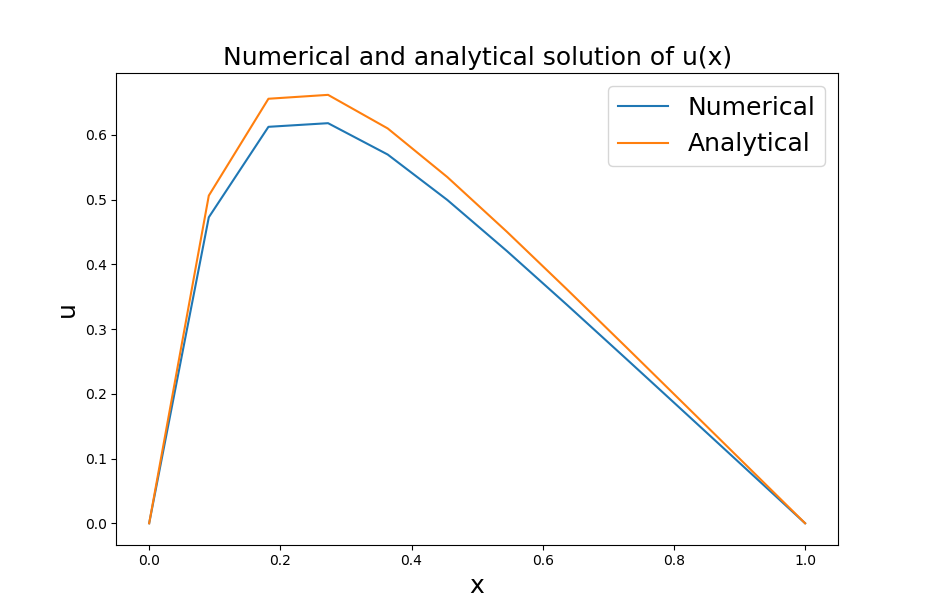
\includegraphics[scale=0.37]{plot1b_n10.png}}}
\qquad
\subfloat[Lowering the step size renders the deviation from the analytical solution invisible in the plot.]{{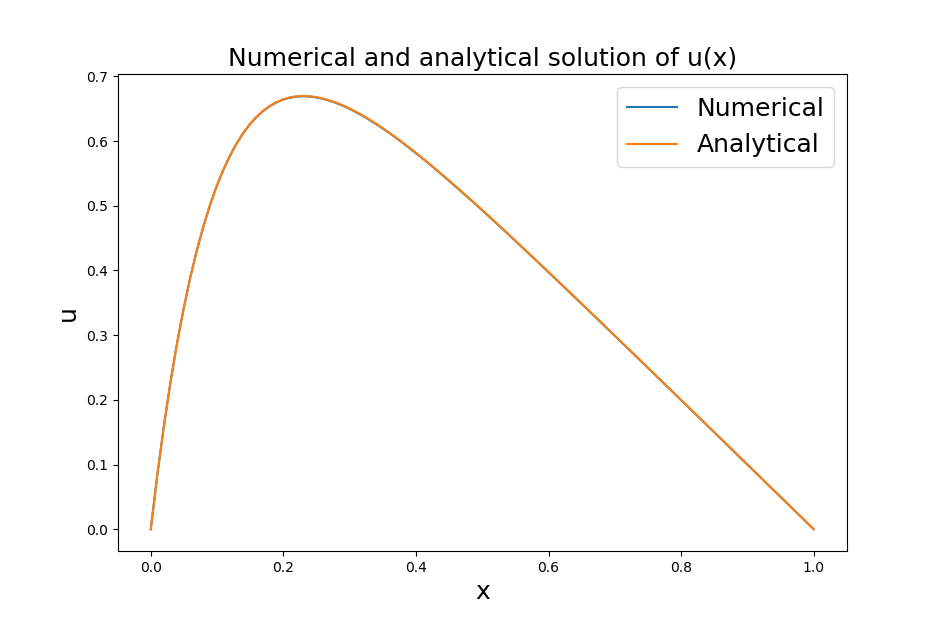
\includegraphics[scale=0.37]{plot1b_n100.png}}}\qquad
\subfloat[Further lowering the step size the only visible difference is in the resolution of the curve in our plot.]{{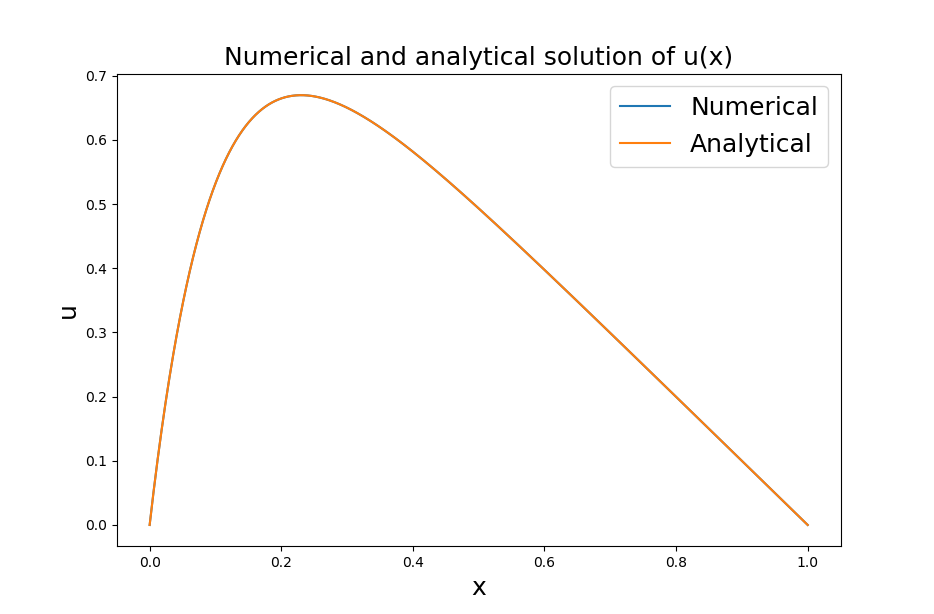
\includegraphics[scale=0.37]{plot1b_n1000.png}}}
\caption{The solution of the differential equation using a generalized algorithm at matrix sizes (a): $n = 10$, (b): $n = 100$ and (c): $n = 1000$.}
\label{fig:fig1}
\end{figure}

\begin{figure}[t]
\mbox{\epsfig{figure=plot1d.png,width=\linewidth,clip=}}
\caption{Logarithmic plot of the error as function of the step size, to illustrate the $\mathcal{O}(h^{2})$ dependency we have plotted $log_{10}(h^{2})=2log_{10}(h)$, which in the plot doubles as $y = 2x$, the expected value of our error.}
\label{fig:fig2}
\end{figure}
%
\begin{deluxetable}{lcc}[H]
%\tablewidth{0pt}
\tablecaption{\label{tab:results}}
\tablecomments{Table of the error, for $n \in [10^1,10^{7}]$ . The table reveals that the numerical error increases when $n > 10^{5}$, while the error for $n \leq 10^{5}$ follow the expected value $\mathcal{O}(h^{2})$.}
\tablecolumns{4}
\tablehead{ n & Error &}
\startdata
 \\
 $10^{1}$ & $6.6114 \cdot 10^{-2}$ &\\
 $10^{2}$ & $8.1651 \cdot 10^{-4}$ &\\
 $10^{3}$ & $8.3167\cdot 10^{-6}$ &\\
 $10^{4}$ & $8.3311\cdot 10^{-8}$ &\\
 $10^{5}$ & $1.4356\cdot 10^{-9}$ &\\
 $10^{6}$ & $8.3973\cdot 10^{-7}$ &\\
 $10^{7}$ & $2.7487\cdot 10^{-6}$ &\\
\enddata
\end{deluxetable}

%
\subsection{Program CPU time}

Testing the time we ran the three different programs 10 times for different sizes $n$, listing longest, shortest and average CPU times.
In Table \ref{tab:n1000} the results we have listed for timing our programs with $n = 1000$. Comparably for larger matrices $n=10^{6}$ the programs yield the timings presented in Table \ref{tab:n10^6}.

\begin{deluxetable}{lccc}[H]
%\tablewidth{0pt}
\tablecaption{\label{tab:n1000}}
\tablecomments{This table contains highest, lowest and average measured CPU times for the different algorithms used at n = 1000, armadillo being overall, while our general and specialized algorithm timings both withing the same order of magnitude.}
\tablecolumns{4}
\tablehead{ & General & Specialized & Armadillo}
\startdata
Highest & 0.000333s & 0.000237s & 0.021747s \\
Lowest & 0.000191s & 0.000074s & 0.012255s  \\
Average & 0.000249s & 0.000167s & 0.015978s 
\enddata
\end{deluxetable}
%

\begin{deluxetable}{lccc}[h]
%\tablewidth{0pt}
\tablecaption{\label{tab:n10^6}}
\tablecomments{This table contains highest, lowest and average measured CPU times for the different algorithms used at $n = 10^{6}$, armadillo runs out of memory, while the general and specialized algorithms staying within the same order of magnitude.}
\tablecolumns{4}
\tablehead{ & General & Specialized & Armadillo}
\startdata
Highest & 0.085026 & 0.073819s & Out of memory \\
Lowest & 0.074668 & 0.064465s & Out of memory  \\
Average & 0.079288s & 0.067805s & Out of memory 
\enddata
\end{deluxetable}
%

Note that the LU-decomposition runs out of memory at $n = 10^{5}$ meaning that we will not be able to test the Armadillo made algorithm for larger matrices. Our general algorithm runs at $8n$ FLOPS, while our specialized algorithm is optimized to only run at $6n$ FLOPS.

\section{Conclusions}
\label{sec:conclusions}
\subsection{Error}
Reviewing the plots from Fig. \ref{fig:fig1} we can see that the error is greater for $n = 10$ than it is for $n = 100$ points. Which is expected of our algorithm considering the error is of the order $h^2$, where $h$ is the step size. However between these step sizes we already reach the maximum resolution of a side by side comparison, and between $n = 100$ and $n = 1000$ the only visible change is in the resolution of the plot itself. Further we compute the relative error of the specialized algorithm compared to the closed form solution and plot it in a logarithmic scale as seen in Fig. \ref{fig:fig2}. By Fig. \ref{fig:fig2} we can see that the error goes as expected until $log_{10}(h) = -5$ and the error increases. This is the point where our numerical model becomes unstable due to the step size being too small, called loss of numerical accuracy, which is a direct result from n being too large.

\subsection{CPU time}
While CPU time of the specialized and the general algorithms are of same order of magnitude, there is a clear difference for $n = 1000$. Analyzing the number of FLOPS in the different algorithms, it becomes clear that the specialized algorithm should be $8n/6n = 3/2$ times faster. Comparing average CPU times we see that this is highly accurate for $n=1000$, in which case its $0.000249/0.000167 = 1.49$times faster. However for $n = 10^{6}$ this does not seem to be the case entirely, as we find it to be $0.079288/0.067805 = 1.17$ times faster. This can partially be attributed to the small sample size and the imprecise method when performing the calculations. The testing environment for calculating was a laptop, we expect that for large n the calculations take more time and there is a higher load on the CPU. This load results in a higher temperature which on a standard laptop could cause the performance to drop.

\subsection{LU decomposition}
The LU decomposition is as expected a slower and more demanding algorithm. Since the algorithm stores the variables as matrices instead of vectors, the computer runs out of memory for larger n i.e $n > 10^{5}$. The reason that the LU decomposition runs out of memory is that it saves every value of the matrix, including the zeros on the lower diagonal $\boldsymbol{L}$ and the upper diagonal of $u$ which takes up a lot of memory when storing the $n\times n$ matrices.
The number of FLOPS using LU decomposition is proportional to $n^{2}$ since we are dealing with $nxn$ matrices. This has a considerable effect and even for smaller n, we get a slower CPU time, due to the large number of FLOPS required in our calculations.

\subsection{Comments}
We both found this project to be great as an introduction to FYS3150 Computational Physics and as a way to start learning C++. We did not have many critiques, other than the fact that in section 1b the variables written in the matrix and the ones in the vector $b$ and $\tilde{b}$ was a bit unclear at first glance, and it is suggested that $\tilde{b}$ in the matrix $\boldsymbol{A}$ is renamed to $\tilde{f}$.




%\begin{figure}[t]
%
%\mbox{\epsfig{figure=filename.eps,width=\linewidth,clip=}}
%
%\caption{Description of figure -- explain all elements, but do not
%draw conclusions here.}
%\label{fig:figure_label}
%\end{figure}


%\lstset{language=python,
%    showspaces=false,
%    extendedchars=true,
%    breaklines=true,
%    tabsize=2,
%    basicstyle=\small\ttfamily,
%    frame=single,
%    columns=flexible,
%    keepspaces=true,
%}
%\begin{lstlisting}
%\end{lstlisting}

%\begin{deluxetable}{lccc}
%\tablewidth{0pt}
%\tablecaption{\label{tab:results}}
%\tablecomments{Summary of main results.}
%\tablecolumns{4}
%\tablehead{Column 1  & Column 2 & Column 3 & Column 4}
%\startdata
%Item 1 & Item 2 & Item 3 & Item 4
%\enddata
%\end{deluxetable}



\begin{acknowledgements}

\end{acknowledgements}

\begin{thebibliography}{}

\bibitem{1}
  M. H. Jensen,
  \textit{Project 1},
  \url{https://github.com/CompPhysics/ComputationalPhysics/blob/master/doc/Projects/2018/Project1/pdf/Project1.pdf} (10.09.18)

\end{thebibliography}


\end{document}
